\documentclass[12pt]{article}

\usepackage{fancyhdr}
\usepackage{geometry}
\usepackage[utf8]{inputenc}
\usepackage[T1]{fontenc}
\usepackage[ngerman]{babel}
\usepackage{amsmath,amssymb,amstext}
\usepackage{hyperref}
\usepackage{cancel}
\usepackage{dsfont}
\usepackage{physics}
\usepackage{lmodern}
\usepackage{enumerate}
\usepackage{enumitem}
\usepackage{graphicx}
\usepackage{listings, color}
\usepackage[labelfont=bf]{caption}
\usepackage{titling}
\usepackage{siunitx}
\usepackage{tikz}
\usepackage{icomma}
\usepackage{revsymb}
\usepackage{pgfplots}
\usepackage[euler]{textgreek}
\usepackage{fixltx2e}
\usepackage{tikz-feynman}
\usepackage{subfigure}

\usepackage[backend=biber,backref=false,style=numeric-comp, sorting=none,block=ragged,firstinits=true]{biblatex}

\lstset{basicstyle=\scriptsize,breaklines=true} %Quellcode mit Umlauten und ganz klein
\lstset{literate=
	{Ö}{{\"O}}1
	{Ä}{{\"A}}1
	{Ü}{{\"U}}1
	{ß}{{\ss}}2
	{ü}{{\"u}}1
	{ä}{{\"a}}1
	{ö}{{\"o}}1
}


%Geometrie----------------------------------------------------------------------------------------------------------

\geometry{a4paper, top=25mm, left=15mm, right=15mm, bottom=25mm,headsep=10mm, footskip=10mm}
\pagestyle{fancy}
\setlength{\parindent}{0pt} %Zeileneinrückung

\fancyhf{} %Setzt voreingestellte Kopf-und Fußzeilen-Eigenschaften zurück

\lhead{\nouppercase{\leftmark}}
\chead{}
\rhead{\thepage}

\lfoot{}
\cfoot{}
\rfoot{}

\title{\vspace{0cm}{\Huge Fortgeschrittenen-Praktikum II:\\ \vspace{1cm} Z\textsuperscript0-Resonanz}}
\author{Saskia Bondza\\Simon Stephan}
\date{durchgeführt vom 13.03.2017 bis 17.03.2017}

\pretitle{%
	\begin{center}
		\LARGE
		
\includegraphics[width=6cm,]{../figures/siegel}\\[\bigskipamount]
	}
	\posttitle{\end{center}}

%neue Commands----------------------------------------------------------------------------------------------------------
\newcommand{\nab}{\vec{\nabla}} %direkter Befehl mit Vektorpfeil
\newcommand{\gra}[3][0.7]{
	\begin{minipage}[h!]{\textwidth}
		\centering
		\includegraphics[width=#1\textwidth]{../figures/#2.png}
		\captionof{figure}{#3}
	\end{minipage}
	\vskip 30 pt
}
\newcommand{\graX}[4][0.7]{
	\begin{minipage}[h!]{\textwidth}
		\centering
		\includegraphics[width=#1\textwidth]{../figures/#2.png}
		\captionof{figure}[#3]{#4}
	\end{minipage}
	\vskip 30 pt
}
\newcommand{\graTwo}[4][0.49]{
	\begin{minipage}[h!]{\textwidth}
		\centering
		\includegraphics[width=#1\textwidth]{../figures/#2.png}
		\includegraphics[width=#1\textwidth]{../figures/#3.png}
		\captionof{figure}{#4}
	\end{minipage}
	\vskip 30 pt
}
\newcommand{\graTwoB}[5]{
	\begin{minipage}[h!]{\textwidth}
		\centering
		\includegraphics[width=#1\textwidth]{../figures/#3.png}
		\includegraphics[width=#2\textwidth]{../figures/#4.png}
		\captionof{figure}{#5}
	\end{minipage}
	\vskip 30 pt
}
\newcommand{\del}[2][]{\frac{\partial #1}{\partial #2}}
\newcommand{\diff}[2][]{\frac{\mathrm d #1}{\mathrm d #2}}
\newcommand{\code}[1]{\texttt{#1}}
\newcommand{\degree}{^\circ}

\newcommand{\vcenterbf}[3][white]{\textcolor{#1}{$P_q$}\textcolor{#2}{\textbf{#3}}\textcolor{#1}{$P_q$}}
\newcommand{\vcenternode}[3][white]{\textcolor{#1}{$P_q$}\textcolor{#2}{#3}\textcolor{#1}{$P_q$}}

\addbibresource{fp_refs.bib}

\renewcommand*{\thesubfigure}{ \alph{subfigure})}

%Titel,Inhalt----------------------------------------------------------------------------------------------------------

\begin{document}
	\pagenumbering{gobble} %verstecke Seitenzahl
	\maketitle
	\newpage
	

	
	\section*{Abstract}
	
	\newpage
	
	\thispagestyle{empty}
	\tableofcontents
	\newpage
	
	%Schreiben----------------------------------------------------------------------------------------------------------
	\pagenumbering{arabic}
	
	\section{Einleitung}
	\newpage
	\section{Theoretische Grundlagen}

\subsection{Standardmodell der Elementarteilchenphysik}

\begin{figure}[bh]
	\centering
	\begin{tikzpicture}
	\node at(0.9,-0.9){\huge\vcenterbf{green}{u}};
	\node at(2.9,-0.9){\huge\vcenterbf{green}{c}};
	\node at(4.9,-0.9){\huge\vcenterbf{green}{t}};
	\node at(0.9,-2.9){\huge\vcenterbf{green}{d}};
	\node at(2.9,-2.9){\huge\vcenterbf{green}{s}};
	\node at(4.9,-2.9){\huge\vcenterbf{green}{b}};
	\node at(0.9,-4.9){\huge\vcenterbf{cyan}{e}};
	\node at(2.9,-4.9){\huge\vcenterbf{cyan}{\textmu}};
	\node at(4.9,-4.9){\huge\vcenterbf{cyan}{\texttau}};
	\node at(0.9,-6.9){\huge \vcenterbf{cyan}{\textnu\textsubscript{e}}};
	\node at(2.9,-6.9){\huge \vcenterbf{cyan}{\textnu\textsubscript{\textmu}}};
	\node at(4.9,-6.9){\huge \vcenterbf{cyan}{\textnu\textsubscript{\texttau}}};
	\node at(6.9,-0.9){\huge\vcenterbf{orange}{\textgamma}};
	\node at(8.9,-0.9){\huge\vcenterbf{red}{H}};
	\node at(6.9,-2.9){\huge\vcenterbf{orange}{g}};
	\node at(6.9,-4.9){\huge\vcenterbf{orange}{Z\textsuperscript{0}}};
	\node at(6.9,-6.9){\huge \vcenterbf{orange}{W$^\pm$}};
	\node at(0.9,-1.65){\scriptsize\vcenternode{green}{up}};
	\node at(2.9,-1.65){\scriptsize\vcenternode{green}{charm}};
	\node at(4.9,-1.65){\scriptsize\vcenternode{green}{top}};
	\node at(0.9,-3.65){\scriptsize\vcenternode{green}{down}};
	\node at(2.9,-3.65){\scriptsize\vcenternode{green}{strange}};
	\node at(4.9,-3.65){\scriptsize\vcenternode{green}{bottom}};
	\node at(0.9,-5.65){\scriptsize\vcenternode{cyan}{Elektron}};
	\node at(2.9,-5.65){\scriptsize\vcenternode{cyan}{Myon}};
	\node at(4.9,-5.65){\scriptsize\vcenternode{cyan}{Tauon}};
	\node at(0.9,-7.65){\scriptsize \vcenternode{cyan}{e-Neutrino}};
	\node at(2.9,-7.65){\scriptsize \vcenternode{cyan}{\textmu-Neutrino}};
	\node at(4.9,-7.65){\scriptsize \vcenternode{cyan}{\texttau-Neutrino}};
	\node at(6.9,-1.65){\scriptsize\vcenternode{orange}{Photon}};
	\node at(8.9,-1.65){\scriptsize\vcenternode{red}{Higgs-Boson}};
	\node at(6.9,-3.65){\scriptsize\vcenternode{orange}{Gluon}};
	\node at(6.9,-5.65){\scriptsize\vcenternode{orange}{Z-Boson}};
	\node at(6.9,-7.65){\scriptsize \vcenternode{orange}{W-Boson}};
	
	\draw[line width=2,color=green] (0,0) rectangle (1.8,-1.8);
	\draw[line width=2,color=green] (2,0) rectangle (3.8,-1.8);
	\draw[line width=2,color=green] (4,0) rectangle (5.8,-1.8);
	\draw[line width=2,color=green] (0,-2) rectangle (1.8,-3.8);
	\draw[line width=2,color=green] (2,-2) rectangle (3.8,-3.8);
	\draw[line width=2,color=green] (4,-2) rectangle (5.8,-3.8);
	\draw[line width=2,color=cyan] (0,-4) rectangle (1.8,-5.8);
	\draw[line width=2,color=cyan] (2,-4) rectangle (3.8,-5.8);
	\draw[line width=2,color=cyan] (4,-4) rectangle (5.8,-5.8);
	\draw[line width=2,color=cyan] (0,-6) rectangle (1.8,-7.8);
	\draw[line width=2,color=cyan] (2,-6) rectangle (3.8,-7.8);
	\draw[line width=2,color=cyan] (4,-6) rectangle (5.8,-7.8);
	\draw[line width=2,color=orange] (6,0) rectangle (7.8,-1.8);
	\draw[line width=2,color=orange] (6,-2) rectangle (7.8,-3.8);
	\draw[line width=2,color=orange] (6,-4) rectangle (7.8,-5.8);
	\draw[line width=2,color=orange] (6,-6) rectangle (7.8,-7.8);
	\draw[line width=2,color=red] (8,0) rectangle (9.8,-1.8);
	
	\draw[line width=1,color=black] (0,1) rectangle (5.8,0.2);
	\draw[line width=1,color=black] (6,1) rectangle (9.8,0.2);
	\draw[line width=1,color=green] (-1,0) rectangle (-0.2,-3.8);
	\draw[line width=1,color=cyan] (-1,-4) rectangle (-0.2,-7.8);
	
	\node at(2.9,0.6){Fermionen};
	\node at(7.9,0.6){Bosonen};
	\node[rotate=90,color=green] at(-0.6,-1.9){Quarks};
	\node[rotate=90,color=cyan] at(-0.6,-5.9){Leptonen};
	
	
	\end{tikzpicture}
	\caption{Standardmodell der Elementarteilchenphysik}
	\label{fig:standardmodell}
\end{figure}

Das in Abbildung \ref{fig:standardmodell} dargestellte Standardmodell der Elementarteilchenphysik beschreibt die aktuellen Erkenntnisse der Teilchenphysik. Es beschreibt die uns bisher bekannten Elementarteilchen, sowie deren Wechselwirkungen mit Ausnahme der sehr schwachen Gravitation. Die Elementarteilchen lassen sich nach ihrem Spin in Fermionen und Bosonen einteilen, wobei die Teilchen mit halbzahligem Spin als Fermionen bezeichnet werden, während der Spin der Bosonen ganzzahlig ist.


\subsubsection{Wechselwirkungen}
Das Standardmodell beschreibt drei fundamentale Wechselwirkungen, die elektromagnetische Wechselwirkung, die schwache Wechselwirkung und die starke Wechselwirkung. Diese Wechselwirkungen werden durch den Austausch von Eichbosonen vermittelt. Die Eichbosonen und die Elementarteilchen, welche den Wechselwirkungen unterliegen werden in Abschnitt \ref{sec:elementarteilchen} eingeführt. Zu jeder Wechselwirkung existiert eine Ladung, die elektromagnetische Ladung, die schwache Ladung sowie die Farbladung der starken Wechselwirkung. Einer Wechselwirkung unterliegen nur Teilchen, die eine entsprechende Ladung tragen. Während die elektromagnetische Wechselwirkung eine unbegrenzte Reichweite hat, ist die Reichweite der schwachen und der starken Wechselwirkung kleiner als ein Atomkernradius. Die starke Wechselwirkung ermöglicht den Aufbau von Hadronen aus Quarks, welche als einige Teilchen der starken Wechselwirkung unterliegen, während die schwache Wechselwirkung für viele Zerfälle und Umwandlungen von Teilchen verantwortlich ist. Wechselwirkungen zwischen Atomen liegt die elektromagnetische Wechselwirkung zu Grunde.

\subsubsection{Elementarteilchen}\label{sec:elementarteilchen}
Fermionen und aus ihnen aufgebaute Teilchen werden als Materie bezeichnet. Die elementaren Fermionen, die Grundbausteine der Materie, lassen sich wiederum in Quarks und Leptonen einteilen. 
\paragraph{Quarks} Als Quarks werden die sechs elemntaren Fermionen bezeichnet, welche eine Farbladung tragen. Die elektromagnetische Ladung der oberen Quarks (up-, charm-, und top-Quark) beträgt $Q=\frac23$, wohingegen die unteren Quarks (down-, strange- und bottom-Quark) die Ladung $Q=\frac13$ tragen. Zu jedem Quark existiert ein Antiquark mit der entgegengesetzten Ladung ($Q_{\bar{q}}=-Q_q$).
\paragraph{Leptonen} Die übrigen elementaren Fermionen werden als Leptonen bezeichnet. Man unterscheidet hier zwischen den geladenen Leptonen (Elektron, Myon und Tauon) mit einer elektromagnetischen Ladung $Q=-1$ und den ungeladenen Leptonen, den sogenannten Neutrinos mit einer elektromagnetischen Ladung $Q=0$. Es lässt sich jedem geladenen Lepton ein dazugehöriges Neutrino zuordnen. Zu jedem Lepton existiert ein Antiteilchen. Die Antiteilchen der geladenen Leptonen haben jeweils die Ladung $Q=1$. Die Antineutrinos sind wie die Neutrinos neutral geladen.
\paragraph{Eichbosonen}
Die Bosonen lassen sich in Vektorbosonen (Spin $S=1$) und skalare Bosonen (Spin $S=0$) unterteilen. Die Vektorbosonen sind die Austauschteilchen der Wechselwirkungen, sogenannte Eichbosonen, während das einzige skalare Boson das Higgs-Boson ist. Die elektromagnetische Wechselwirkung wird über das Photon übertragen, das Gluon ist das Austauschteilchen der starken Wechselwirkung und die Eichbosonen der schwachen Wechselwirkung sind das geladene $W^\pm$- und das ungeladene $Z^0$-Boson.

\subsubsection{Elektroschwache Wechselwirkung}

%Zusammenhang zwischen elektro und schwach
%Weinbergwinkel

%Saskia

\subsection{Das Z\textsuperscript0-Boson}

Wie in Abschnitt \ref{sec:elementarteilchen} erwähnt, existieren drei Eichbosonen der schwachen Wechselwirkung. Die geladenen Eichbosonen $W^+$ und $W^-$ spielen beispielsweise eine wichtige Rolle für den $\beta$-Zerfall. Ein Neutron zerfällt in ein Proton, in dem sich ein down-Quark unter Aussendung eines $W^-$ in einen up-Quark umwandelt. Das $W^-$ zerfällt daraufhin in ein Elektron und ein Anti-Elektron-Neutrino. Das $W^\pm$ erzeugt also Übergänge mit Ladungsänderung.\\

Es sind jedoch auch neutrale, ladungserhaltende Prozesse in der schwachen Wechselwirkung möglich. Diese werden durch den Austausch eines $Z^0$-Bosons durchgeführt. Das $Z^0$-Boson entsteht beispielsweise durch die Kollision von Elektronen und Positronen, den Antiteilchen des Elektrons mit einer Schwerpunktsenergie nahe der Masse des $Z^0$-Bosons. Anschließend zerfällt es in beliebige $f\bar{f}$-Paare, wobei $f$ für ein beliebiges Fermion und $\bar{f}$ für das dazugehörige Antiteilchen steht.

\subsection{e$^+$e$^-$-Prozesse}\label{sec:e+e-}

In diesem Versuch werden Daten von Elektron-Positron-Kollisionen ausgewertet. Bei dieser Kollision sind die folgenden verschiedenen Prozesse möglich.
\paragraph{Paarvernichtung und Erzeugung von Photonen}
Bei der Kollision von Elektron und Positron können diese sich annihilieren und dabei in zwei oder drei reelle Photonen zerfallen. Die Energie der Teilchen wird dabei vollständig an die Photonen übertragen. Dieser Prozess ist in Abbildung \ref{fig:feynmanphotonen} dargestellt. Bei diesem Prozess ist kein $Z^0$-Boson beteiligt, weshalb der Prozess in der Auswertung eliminiert werden muss.

\begin{figure}
	\centering
	\begin{tikzpicture}
		\begin{feynman}
			\vertex (em) {$e^-$};
			\vertex [below right=of em](a);
			\vertex [below=of a](b);
			\vertex [below left=of b](ep){$e^+$};
			\vertex [above right=of a](p1){$\gamma$};
			\vertex [below right=of b](p2){$\gamma$};
			
			\diagram{
				(em)--[fermion](a)--[fermion](b)--[fermion](ep),
				(a)--[photon](p1),
				(b)--[photon](p2),
				};
		\end{feynman}
	\end{tikzpicture}
	\caption{Feynman-Graph der Erzeugung zweier Photonen}
	\label{fig:feynmanphotonen}
\end{figure}

\paragraph{Paarvernichtung und Erzeugung eines $Z^0$-Bosons}
Bei der Annihilation des Elektron-Positron-Paares kann ein virtuelles Photon und bei entsprechender Schwerpunktsenergie ein $Z^0$-Boson erzeugt werden. Dieses wiederum zerfällt nun in ein beliebiges $f\bar f$-Paar. In Abbildung \ref{fig:feynmanz0} ist dieser Prozess dargestellt.

\begin{figure}
	\centering
	\begin{tikzpicture}
	\begin{feynman}
	\vertex (em) {$e^-$};
	\vertex [below right=of em](a);
	\vertex [right=of a](b);
	\vertex [below left=of a](ep){$e^+$};
	\vertex [above right=of b](f1){$\bar f$};
	\vertex [below right=of b](f2){$f$};
	
	\diagram{
		(em)--[fermion](a)--[fermion](ep),
		(a)--[boson,edge label={$\gamma, Z^0$}](b),
		(f1)--[fermion](b)--[fermion](f2),
	};
	\end{feynman}
	\end{tikzpicture}
	\caption{Feynman-Graph der Erzeugung eines Z\textsuperscript0-Bosons}
	\label{fig:feynmanz0}
\end{figure}

\paragraph{Bhabha-Streuung}
Die Bhabha-Streuung beschreibt den Prozess $e^+e^-\rightarrow e^+e^-$. Zusätzlich zur oben beschrieben Annihilation muss hier noch die elastische Streuung von Elektron und Positron unter Austausch eines virtuellen Photons oder $Z^0$-Bosons betrachtet werden. Die Bhabha-Streuung ist in Abbildung \ref{fig:feynmanbhabha} dargestellt.


\begin{figure}
	\centering
	\begin{tikzpicture}
		\begin{feynman}
		\vertex (ep) {$e^+$};
		\vertex [below right=of ep](a);
		\vertex [right=of a](b);
		\vertex [below left=of a](em){$e^-$};
		\vertex [above right=of b](f1){$e^+$};
		\vertex [below right=of b](f2){$e^-$};
		
		\diagram{
			(ep)--[fermion](a)--[fermion](em),
			(a)--[boson,edge label={$\gamma, Z^0$}](b),
			(f1)--[fermion](b)--[fermion](f2),
		};
		\end{feynman}
	\end{tikzpicture}
	\begin{tikzpicture}
		\begin{feynman}
		\vertex (ep) {$e^+$};
		\vertex [below right=of ep](a);
		\vertex [below=of a](b);
		\vertex [below left=of b](em){$e^-$};
		\vertex [above right=of a](f1){$e^+$};
		\vertex [below right=of b](f2){$e^-$};
		
		\diagram{
			(f1)--[fermion](a)--[fermion](ep),
			(a)--[boson,edge label={$\gamma, Z^0$}](b),
			(em)--[fermion](b)--[fermion](f2),
		};
		\end{feynman}
	\end{tikzpicture}
	\caption[Feynman-Graphen der Bhabha-Streuung]{Feynman-Graphen der Bhabha-Streuung (links: s-Kanal; rechts: t-Kanal)}
	\label{fig:feynmanbhabha}
\end{figure}

\paragraph{Inelastische Streuung}
Bei der inelastischen Streuung werden zwei virtuelle Photonen ausgesendet, welche anschließend durch Interaktion ein Hadron erzeugen. Der Prozess der inelastischen Streuung wird in Abbildung \ref{fig:feynmaninelastisch} dargestellt. Bei diesem Prozess ist kein $Z^0$-Boson beteiligt, weshalb der Prozess in der Auswertung eliminiert werden muss.

\begin{figure}
	\centering
	\begin{tikzpicture}
	\begin{feynman}
	\vertex (em) {$e^-$};
	\vertex [below right=of em](a);
	\vertex [below right=of a](p);
	\vertex [below left=of p](b);
	\vertex [below left=of b](ep){$e^+$};
	\vertex [right=of p](h){$h$};
	
	\diagram{
		(em)--[fermion](a)--[fermion](b)--[fermion](ep),
		(a)--[photon,edge label=$\gamma$](p),
		(b)--[photon,edge label'=$\gamma$](p),
		(p)--(h),
	};
	\end{feynman}
	\end{tikzpicture}
	\caption{Feynman-Graph der inelastischen Streuung}
	\label{fig:feynmaninelastisch}
\end{figure}

\subsection{Z\textsuperscript0-Resonanz}

Die Prozesse, welche die Erzeugung eines $Z^0$-Bosons beinhalten sind jeweils nur im Bereich um die Masse des $Z^0$-Bosons möglich. Durch Untersuchung dieser Prozesse bei unterschiedlichen Schwerpunktsenergien rund um die erwartete Masse des $Z^0$-Bosons lässt sich nun die genaue Masse sowie die Zerfallsbreite des $Z^0$-Bosons bestimmen. Erwartet wird ein Resonanzmaximum des Wirkungsquerschnitts bei der Masse $M_Z$ des $Z^0$-Bosons.

\subsubsection{Bhabha-Streuung}\label{sec:bhabha}

Wie bereits in Abschnitt \ref{sec:e+e-} beschrieben, tragen zwei Feynman-Graphen zur Bhabha-Streuung bei (siehe Abbildung \ref{fig:feynmanbhabha}). Der s-Kanal beschreibt den Beitrag des Vernichtungsprozesses, während der t-Kanal Streuprozesse beschreibt. Für die Messung der Zerfallsbreite des $Z^0$-Bosons ist also nur der s-Kanal relevant. Unterscheiden lassen sich die unterschiedlichen Prozesse am Streuwinkel $\theta$ zwischen dem einlaufenden und dem auslaufenden Elektron. Für große Winkel dominiert der s-Kanal, für kleine Winkel der t-Kanal. Die Winkelabhängigkeit des Wirkungsquerschnitts wird durch folgende Formel beschrieben:
\begin{align}
	\del[\sigma]{\Omega}&=s\cdot\left(1+\cos^2\theta\right)+t\cdot\left(1-\cos\theta\right)^{-2}\text{.}\label{eq:stkanal}
\end{align}

\begin{figure}
	\centering
	\begin{tikzpicture}
	\begin{axis}[
	width=0.9\textwidth,
	height=0.5\textwidth,
	axis lines=left, 
	xlabel=$\cos\theta$, 
	ylabel=$\frac{\partial \sigma}{\partial \theta}\,/\,\si{nb}$,
	ymajorgrids=true,
	xmajorgrids=true,
	grid style=dotted,
	legend pos=north west
	]
	\addplot[domain=-1:0.9,samples=1000,color=green,line width=2]
	{0.1*(1-x)^(-2)};
	\addlegendentry{t-Kanal};
	\addplot[domain=-1:0.9,samples=1000,color=blue,line width=2]
	{1*(1+x^2)};
	\addlegendentry{s-Kanal};
	\addplot[domain=-1:0.9,samples=1000,color=red,line width=2,style=dashed]
	{1*(1+x^2)+0.1*(1-x)^(-2)};
	\addlegendentry{Gesamt};
	\end{axis}
	\end{tikzpicture}
	\caption[Bhabha-Wirkungsquerschnitt für t-Kanal und s-Kanal]{Bhabha-Wirkungsquerschnitt für t-Kanal und s-Kanal.}
	\label{fig:winkelbhabhatheorie}
\end{figure}

\subsubsection{Annihilation in Fermionenpaare}
Die Paarvernichtung mit anschließendem Zerfall in ein $f\bar f$-Paar ist durch ein Photon oder ein $Z^0$-Boson möglich. Relevant für diesen Versuch ist nur der Zerfall durch das $Z^0$-Boson. Der Wirkungsquerschnitt in Abhängigkeit der Schwerpunktsenergie $E=\sqrt{s}$ ist gegeben durch eine Breit-Wigner-Verteilung:
\begin{align}
	\sigma_f(s)&=\frac{12\pi}{M_Z^2}\frac{s\Gamma_e\Gamma_f}{\left(s-M_Z^2\right)^2+\left(s\frac{\Gamma_Z}{M_z}\right)^2}\text{.}
\end{align}
Hierbei beschreibt $\Gamma_e$ die Zerfallsbreite des Elektrons, $\Gamma_f$ die Zerfallsbreite des Fermions und $\Gamma_Z$ die Gesamtbreite.

\subsubsection{Berechnung der Zerfallsbreiten}\label{sec:partialbreiten}

Die Partialbreiten der Zerfallskanäle berechnen sich nach \cite{anleitungalt} folgendermaßen:

\begin{align}
	\Gamma_f&=\frac{N_c^f\sqrt2}{12\pi}\cdot G_FM_Z^3\left(\left(g_v^f\right)^2+\left(g_A^f\right)^2\right)\label{eq:partialbreiten}
\end{align}
mit \cite{anleitungalt,nakamura}:
\begin{align}
	N_c^f&=
	\begin{cases}
		1&\text{für } f\in\{e, \mu, \tau, \nu_e, \nu_\mu, \nu_\tau\}\\
		3&\text{für } f\in\{u, d, c, s, b\}
	\end{cases}\text{,}\\
	G_F&=(1,66370\pm0,00010)\cdot10^{-5}\,\si{GeV^{-2}}\text{,}\\
	M_Z&=(91,188\pm0,002)\,\si{GeV}\text{,}\\
	g_v^f&=I_3^f-2Q_f\sin^2\left(\theta_W\right)\text{,}\\
	g_A^f&=I_3^f\text{,}\\
	I_3^f&=
	\begin{cases}
		-\frac12&\text{für } f\in\{e, \mu, \tau, d, s, b\}\\
		\frac12&\text{für } f\in\{\nu_e, \nu_\mu, \nu_\tau, u, c\}
	\end{cases}\text{,}\\
	Q_f&=
	\begin{cases}
		-1&\text{für } f\in\{e, \mu, \tau\}\\
		-\frac13&\text{für } f\in\{d, s, b\}\\
		0&\text{für } f\in\{\nu_e, \nu_\mu, \nu_\tau\}\\
		\frac23&\text{für } f\in\{u, c\}\footnotemark
	\end{cases}\text{,}\\
	\sin^2\left(\theta_W\right)&=0,23116\pm0,00013\text{.}
\end{align}
\footnotetext{Der Zerfall in $\tau\bar\tau$ ist aufgrund der hohen Masse des Top-Quarks nicht möglich.}

Aus Gleichung \ref{eq:partialbreiten} ergeben sich folgende Ergebnisse:
\begin{alignat}{3}
	&\Gamma_{e/\mu/\tau}&&=&(83,412\pm0,009)\,\si{MeV}\text{,}\label{eq:leptonenuniversalitaet}\\
	&\Gamma_{\nu_e/\nu_\mu/\nu_\tau}&&=&\,(165,884\pm0,011)\,\si{MeV}\text{,}\label{eq:neutrinos}\\
	&\Gamma_{d/s/b}&&=&(367,91\pm0,06)\,\si{MeV}\text{,}\\
	&\Gamma_{u/c}&&=&(285,43\pm0,07)\,\si{MeV}\text{.}
\end{alignat}
Daraus lassen sich nun die gesamte Zerfallsbreite $\Gamma_Z$, die hadronische Zerfallsbreite $\Gamma_q$, die geladene leptonische Zerfallsbreite $\Gamma_l$ und die Neutrino-Zerfallsbreite $\Gamma_\nu$ zu folgenden Werten bestimmen:
\begin{alignat}{3}
	&\Gamma_Z&&=&(2422,5\pm0,2)\,\si{MeV}\text{,}\\
	&\Gamma_q&&=&\,(1674,59\pm0,19)\,\si{MeV}\text{,}\\
	&\Gamma_l&&=&(250,24\pm0,03)\,\si{MeV}\text{,}\\
	&\Gamma_\nu&&=&(497,65\pm0,03)\,\si{MeV}\text{.}
\end{alignat}

Der Wirkungsquerschnitt $\sigma_f$ zur Erzeugung eines $f\bar{f}$-Paars bei der Schwerpunktenergie $\sqrt{s}$ ist gegeben durch:
\begin{align}
	\sigma_f&=\frac{12\pi}{M_Z^2}\frac{s\Gamma_e\Gamma_f}{\left(s-M_Z^2\right)^2+\left(s\frac{\Gamma_Z}{M_Z}\right)^2}
\end{align}
und ergibt sich am Resonanzmaximum ($\sqrt{s}=M_z$) zu
\begin{align}
	\sigma_f^\text{Peak}&=\frac{12\pi}{M_Z^2}\frac{\Gamma_e}{\Gamma_Z}\frac{\Gamma_f}{\Gamma_Z}\text{.}
\end{align}

\begin{figure}
	\centering
	\begin{tikzpicture}
		\begin{axis}[
			width=0.9\textwidth,
			height=0.5\textwidth,
			axis lines=left, 
			xlabel=$\sqrt{s}\,/\,\si{GeV}$, 
			ylabel=$\sigma_f\,/\,\si{nb}$,
			ymajorgrids=true,
			xmajorgrids=true,
			grid style=dotted,
			ymin=0,ymax=45,
			xmin=84,xmax=98
		]
			\addplot[domain=80:100,samples=1000,color=red,line width=2]
			{0.3894*10^6*12*3.14159265359/(91.188^2)*x^2*0.083412*0.25024/((x^2-91.188^2)^2+x^4*(2.4225/91.188)^2)};
			\addlegendentry{Leptonen};
			\addplot[domain=80:100,samples=1000,color=green,line width=2]
			{0.3894*10^6*12*3.14159265359/(91.188^2)*x^2*0.083412*0.49765/((x^2-91.188^2)^2+x^4*(2.4225/91.188)^2)};
			\addlegendentry{Neutrinos};
			\addplot[domain=80:100,samples=1000,color=blue,line width=2]
			{0.3894*10^6*12*3.14159265359/(91.188^2)*x^2*0.083412*1.67459/((x^2-91.188^2)^2+x^4*(2.4225/91.188)^2)};
			\addlegendentry{Quarks};
		\end{axis}
	\end{tikzpicture}
	\caption[Partielle Wirkungsquerschnitte in Abhängigkeit der Schwerpunktsenergie]{Partielle Wirkungsquerschnitte in Abhängigkeit der Schwerpunktsenergie.}
	\label{fig:partialbreiten}
\end{figure}

Der Verlauf der Wirkungsquerschnitte für Leptonen, Neutrinos und Quarks ist in Abbildung \ref{fig:partialbreiten} dargestellt. Wir erhalten folgende partielle Wirkungsquerschnitte am Resonanzmaximum:
\begin{alignat}{3}
	&\sigma_q^\text{Peak}&&=&(42,022\pm0,010)\,\si{nb}\text{,}\\
	&\sigma_l^\text{Peak}&&=&\,(6,2794\pm0,0013)\,\si{nb}\text{,}\\
	&\sigma_{e/\mu/\tau}^\text{Peak}&&=&(2,0931\pm0,0006)\,\si{nb}\text{,}\\
	&\sigma_\nu^\text{Peak}&&=&(12,488\pm0,003)\,\si{nb}\text{,}
\end{alignat}
wobei $\sigma_{e/\mu/\tau}$ der Wirkungsquerschnitt eines einzelnen Leptons ist, während $\sigma_{l}$ der Wirkungsquerschnitt für alle geladenen Leptonen ist, so wie $\sigma_\nu$ der Wirkungsquerschnitt für alle Neutrinos ist.

\paragraph{Weitere Leptonengeneration} Falls der Zerfall des $Z^0$-Bosons in ein weiteres Lepton $x$ möglich ist, sind zwei zusätzliche Zerfallskanäle zu betrachten: $Z^0\rightarrow x\bar x$ und $Z^0\rightarrow \nu_x\bar{\nu}_x$. Nach Gleichung \ref{eq:partialbreiten} gilt dann:
\begin{alignat}{6}
	&\Gamma_x&&=\Gamma_{e/\mu/\tau}&&=&\,(83,412\pm\,0,009)\,\si{MeV}\text{,}\\
	&\Gamma_{\nu_x}&&=\Gamma_{\nu_e/\nu_\mu/\nu_\tau}&&=&\,(165,884\pm\,0,011)\,\si{MeV}\text{.}
\end{alignat}
Die relative Änderung der Zerfallsbreite beträgt also:
\begin{align}
	p&=\frac{\Delta\Gamma_Z}{\Gamma_Z}=\frac{\Gamma_x+\Gamma_{\nu_x}}{\Gamma_Z}=(10,2910\pm0,0010)\,\%\text{.}
\end{align}

\subsection{Vorwärts-Rückwärts-Asymmetrie}\label{sec:asymm}
Die Vorwärts-Rückwärts-Asymmetrie beschreibt den Unterschied der Wirkungsquerschnitte für Winkel $\theta>0$ und Winkel $\theta<0$. Sie ist definiert durch \cite{anleitungalt}:
\begin{align}
	A_{FB}&=\frac{\int\limits_0^1\del[\sigma]{\cos\theta}\mathrm d\cos\theta
		-\int\limits_{-1}^0\del[\sigma]{\cos\theta}\mathrm d\cos\theta}
	{\int\limits_0^1\del[\sigma]{\cos\theta}\mathrm d\cos\theta
		+\int\limits_{-1}^0\del[\sigma]{\cos\theta}\mathrm d\cos\theta}\text{.}\label{eq:asymm}
\end{align}

Nach der Born'schen Näherung gilt für den differentiellen Wirkungsquerschnitt der Reaktion $e^+e^-\rightarrow f\bar f$ \cite{anleitungalt}:
\begin{align}
	\diff[\sigma]{\Omega}&=\frac{\alpha^2\cdot N_c^f}{4s}\left(F_1(s)\cdot\left(1+\cos^2\theta\right)+2F_2(s)\cdot\cos\theta\right)\text{.}
\end{align}
Daraus ergibt sich für die Asymmetrie:
\begin{align}
	A_{FB}&=\frac34\frac{F_2}{F_1}\text{.}
\end{align}
Am Resonanzmaximum ergibt sich das zu \cite{anleitungalt}:
\begin{align}
	A_{FB}^{\mathrm{Peak}}&=3\left(1-4\sin^2\theta_W\right)^2\text{,}\label{eq:weinberg}
\end{align}
mit dem Weinbergwinkel $\theta_W$, welcher sich somit aus der Vorwärts-Rückwärts-Asymmetrie berechnen lässt.

\subsection{Strahlungskorrekturen}
%Simon

\subsection{Teilchendetektoren}
%Saskia

\subsection{Monte-Carlo-Simulation}
\label{sec:montecarlo}
%Saskia


	\newpage
	\section{Durchführung}
	\newpage
	\section{Auswertung}

\subsection{Teilchenidentifikation}

\begin{figure}[h]
	\centering
	\subfigure[Elektronen]{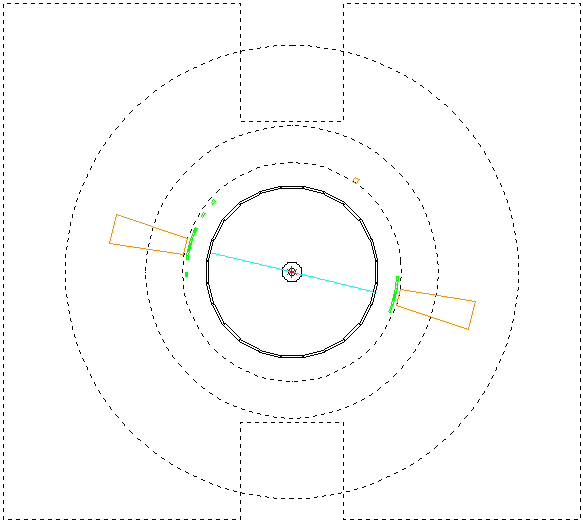
\includegraphics[width=0.49\textwidth]{../figures/grope-ee-w.png}}
	\subfigure[Myonen]{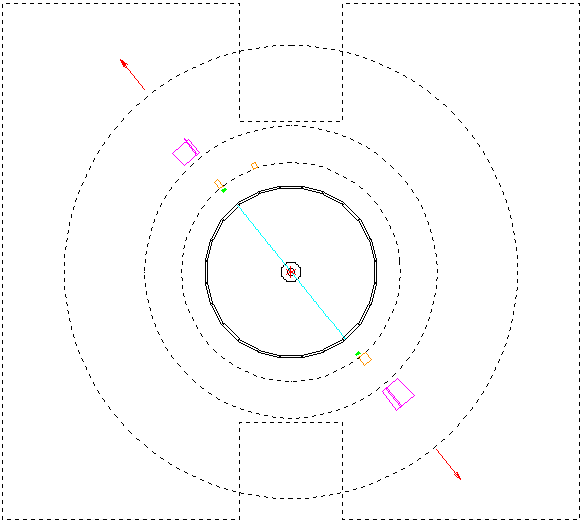
\includegraphics[width=0.49\textwidth]{../figures/grope-mm-w.png}}
	\subfigure[Tauonen]{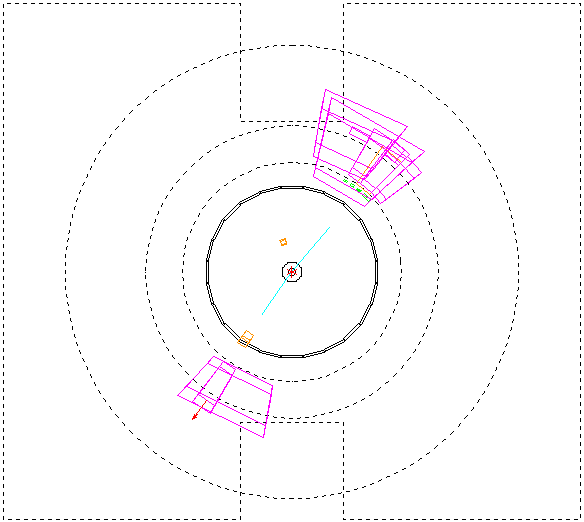
\includegraphics[width=0.49\textwidth]{../figures/grope-tt-w.png}}
	\subfigure[Quarks]{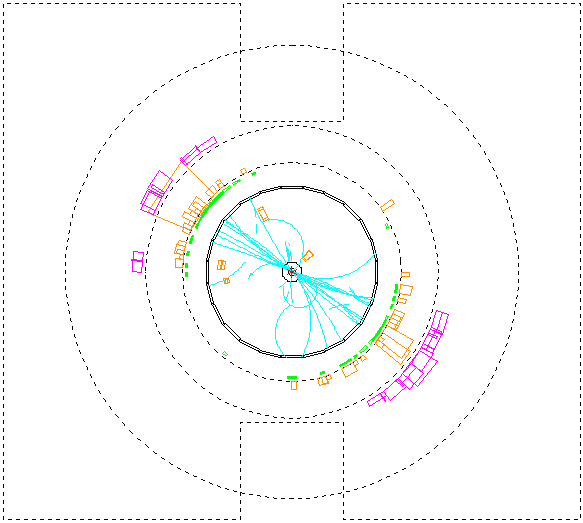
\includegraphics[width=0.49\textwidth]{../figures/grope-qq-w.png}}
	\caption[Detektor-Simulationen für die erwarteten Zerfallsprozesse des Z\textsuperscript0-Bosons]{Detektor-Simulationen für die erwarteten Zerfallsprozesse des Z\textsuperscript0-Bosons. Die Bilder wurden mit GROPE aufgenommen und mit GIMP zur besseren Sichtbarkeit bearbeitet.}
	\label{fig:grope}
\end{figure}
Um später die Separation der Zerfallskanäle durchführen zu können, werden zunächst die einzelnen Zerfallskanäle simuliert und betrachtet. In Abbildung \ref{fig:grope} ist für jeden Zerfallskanal ein Prozess beispielhaft dargestellt.\\

\begin{figure}
	\centering
	\subfigure[$N_\mathrm{charged}$]{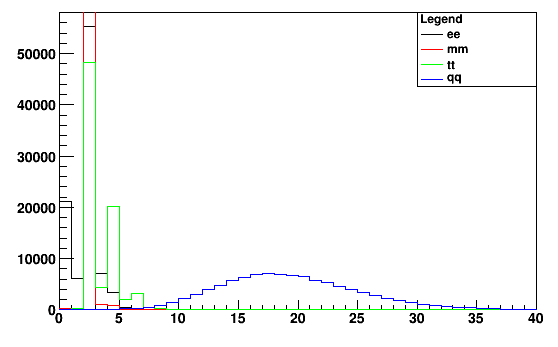
\includegraphics[width=0.49\textwidth]{../figures/Ncharged.png}}
	\subfigure[$P_\mathrm{charged}$]{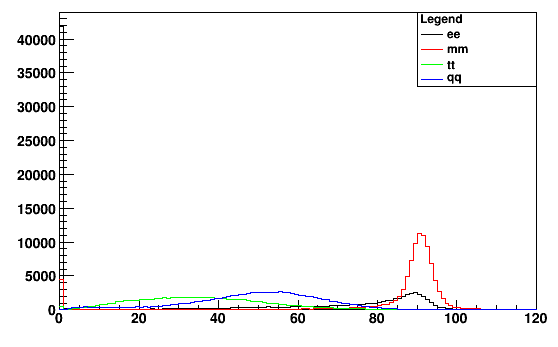
\includegraphics[width=0.49\textwidth]{../figures/Pcharged.png}}
	\subfigure[$E_\mathrm{ecal}$]{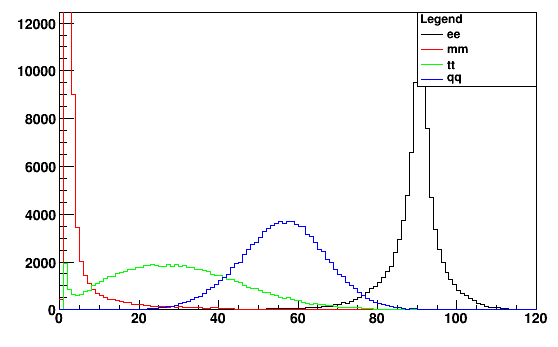
\includegraphics[width=0.49\textwidth]{../figures/E_ecal.png}}
	\subfigure[$E_\mathrm{hcal}$]{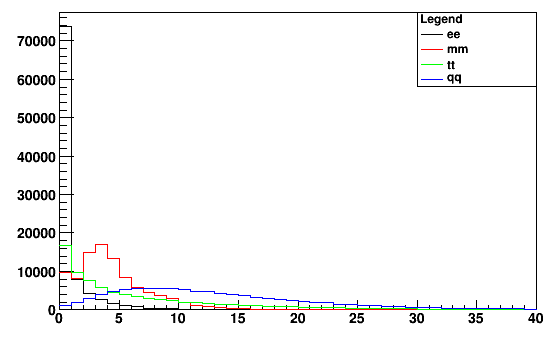
\includegraphics[width=0.49\textwidth]{../figures/E_hcal.png}}
	\subfigure[$\cos\theta$]{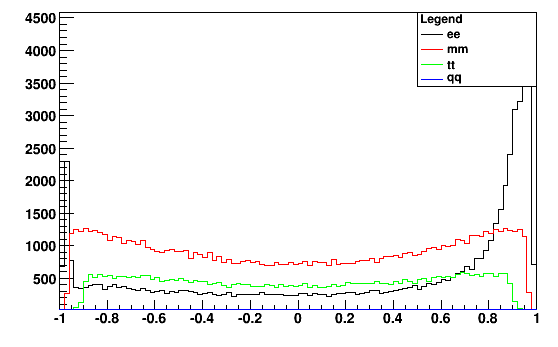
\includegraphics[width=0.49\textwidth]{../figures/cos_thet.png}}
	\caption[Verteilungen der Parameter für die Monte-Carlo-simulierten Daten]{Verteilungen der Parameter für die Monte-Carlo-simulierten Daten.}
	\label{fig:mc}
\end{figure}

Jeder Zerfall lässt sich durch bestimmte Parameter charakterisieren. Dies sind die Anzahl $N_\text{charged}$ der geladenen Spuren im Spurdetektor, $P_\text{charged}$ der Impuls der geladenen Teilchen im Spurdetektor, $E_\text{ecal}$ die an das elektromagnetische Kalorimeter abgegebene Energie, $E_\text{hcal}$ die an das hadronische Kalorimeter abgegebene Energie und $\cos\theta$ der Winkel zwischen einlaufenden und auslaufenden Teilchen. Mit Hilfe der Monte-Carlo-Simulation (siehe Abschnitt \ref{sec:montecarlo}) lassen sich diese Parameter für die einzelnen Zerfallskanäle separat simulieren. Die einzelnen Parameter sind in Abbildung \ref{fig:mc} aufgetragen.\\

Aus diesen Daten lassen sich nun Schnitte festlegen, nach denen die einzelnen Zerfallskanäle aus den experimentell erhaltenen Daten separiert werden können. Zum Festlegen der Schnitte wurde das Skript \code{makeCuts.C} im Anhang \ref{sec:root} entwickelt. Die hierbei vorläufig festgelegten Schnitte sind in Tabelle \ref{tab:cuts} zu finden.

\paragraph{Effizienz und Reinheit}
Um die Güte eines festgelegten Schnittes zu bestimmen, lassen sich zwei Größen berechnen: Dies sind die Effizienz $\mathcal{E}_f^i$ und die Reinheit $p_f^i$ des Schnittes $i$ für den Zerfallskanal $f$. Diese Größen sind wie folgt definiert:
\begin{align}
	\mathcal{E}_f^i&=\frac{N_f^i}{N_i}\\
	p_f^i&=1-\frac{\sum\limits_{j\neq f}N_j^i\cdot \mathrm{BR}_j}{\sum\limits_{j}N_j^i\cdot \mathrm{BR}_j}\text{.}
\end{align}

Die Effizienz beschreibt dabei den Anteil der Fermionen $f$, welche sich innerhalb des Cuts befinden, an der Gesamtanzahl der Fermionen $f$, während die Reinheit den Anteil der Fermionen $f$, welche sich innerhalb des Cuts befinden, an der Gesamtanzahl aller Teilchen, welche sich innerhalb des Cuts befinden, beschreibt.\\

Offensichtlich sind die theoretisch optimale Effizienz und Reinheit gegeben durch:
\begin{align}
	\mathcal{E}_f^i&=\delta_{if}\\
	p_f^i&=\delta_{if}
\end{align}

Die theoretisch optimalen Werte können natürlich im Experiment nicht erreicht werden. Ziel bei der Festlegung der Schnitte ist es jedoch, für beide Größen möglichst hohe Werte zu erzielen.

\begin{table}
	\centering
	\begin{tabular}{r|p{10 cm}}
		\textbf{Zerfallskanal}&\textbf{Schnitt}\\\hline
		Elektronen&$\left(N_\text{charged}<5 \land E_\text{ecal}\geq74\right) \lor \left(P_\text{charged}=0\land E_\text{ecal}>80\right)$\\
		Myonen&$N_\text{charged}<5 \land E_\text{ecal}<50 \land \left(P_\text{charged}\geq 75 \lor P_\text{charged}<1\right)$\\
		Tauonen&$N_\text{charged}<5 \land E_\text{ecal}<74 \land P_\text{charged}< 75$\\
		Quarks&$N_\text{charged}>7$\\
	\end{tabular}
	\caption{Vorläufig festgelegte Schnitte zur Separation der Zerfallskanäle}
	\label{tab:cuts}
\end{table}

\paragraph{2-Photonen-Prozesse}
Ein in der Simulation nicht berücksichtigter Prozess ist der in \ref{sec:e+e-} beschriebene Prozess der inelastischen Streuung, auch als 2-Photonen-Prozess bezeichnet. Um diese zu eliminieren betrachtet man, wie in Abbildung \ref{fig:2photon} beispielhaft für den elektronischen Zerfallskanal dargestellt, die (normierte) Anzahl an Ereignissen in Abhängigkeit von $P_\text{charged}$ und $E_\text{ecal}$ sowohl der experimentellen als auch der simulierten Daten. Nun sucht man Stellen, an denen in den experimentellen Daten deutlich mehr Ereignisse auftauchen als in den simulierten Daten. Diese sind dann vermutlich auf solche 2-Photonen-Prozesse zurückzuführen und lassen sich durch eine Anpassung der Schnitte eliminieren. Im Rahmen der 2-Photonen-Korrektur wurden die Schnitte der Elektronen und der Tauonen angepasst, in dem jeweils eine zusätzliche Grenze $P_\text{charged}>15$ hinzugefügt wurde.
\begin{figure}
	\centering
	\subfigure[Simulation]{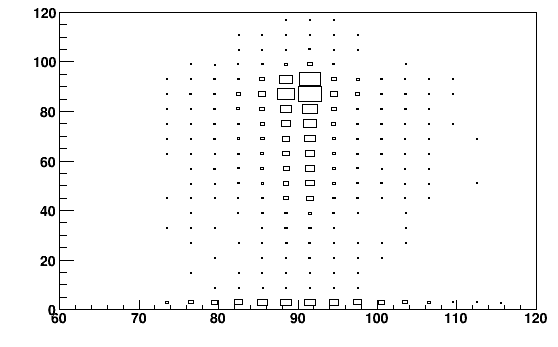
\includegraphics[width=0.49\textwidth]{../figures/ee_2photon_mc.png}}
	\subfigure[Experiment]{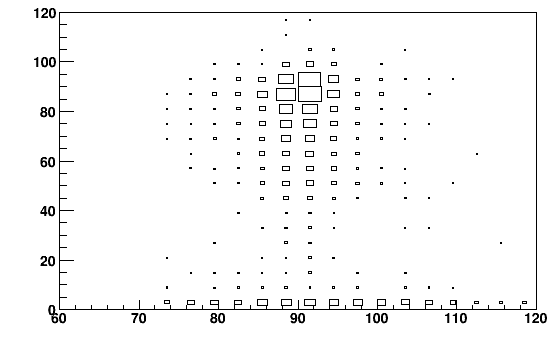
\includegraphics[width=0.49\textwidth]{../figures/ee_2photon_data.png}}
	\caption[Identifizierung der 2-Photon-Ereignisse]{Ereignisse über $P_\text{charged}$ (links) und $E_\text{ecal}$ (unten) zur Identifizierung der 2-Photon-Ereignisse, beispielhaft für Elektronen.}
	\label{fig:2photon}
\end{figure}

\paragraph{Trennung von t-Kanal und s-Kanal}
Wie in Abschnitt \ref{sec:bhabha} beschrieben, existiert für die Elektronen sowohl ein t-Kanal als auch ein s-Kanal, für unseren Versuch ist allerdings nur der s-Kanal relevant. Daher wird die in Abbildung \ref{fig:winkelbhabhatheorie} dargestellte Gleichung \ref{eq:stkanal} an die simulierte $\cos\theta$-Verteilung für Elektronen gefittet und daraus die Parameter $s$ und $t$ bestimmt (siehe Abbildung \ref{fig:stkanal}). Anhand des Fits kann nun eine Obergrenze für $\cos\theta$ festgelegt und der Schnitt entsprechend angepasst werden. Die Obergrenze wurde hier bei $\cos\theta=0.4$ gewählt.

\begin{figure}
	\centering
	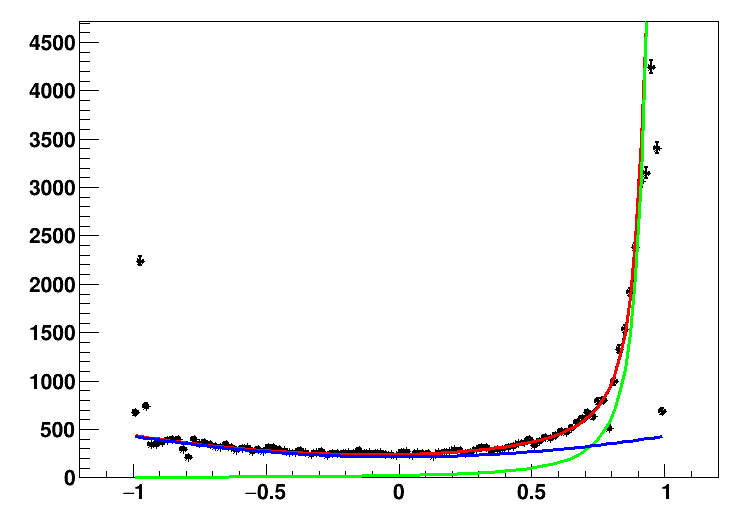
\includegraphics[width=0.8\textwidth]{../figures/stkanal.png}
	\caption[$\cos\theta$-Verteilung für Elektronen mit Fit des erwarteten Verlaufs]{$\cos\theta$-Verteilung für Elektronen mit Fit des erwarteten Verlaufs (rot). Außerdem eingezeichnet sind separat der s-Kanal (blau) und der t-Kanal (grün)}
	\label{fig:stkanal}
\end{figure}

\paragraph{Endgültige Festlegung der Schnitte}
Anhand der Korrekturen durch 2-Photonen-Prozesse und den Einfluss der t-Kanal-Prozesse können nun die Schnitte entsprechend Tabelle \ref{tab:finalcuts} festgelegt werden.

\begin{table}
	\centering
	\begin{tabular}{r|p{11 cm}}
		\textbf{Zerfallskanal}&\textbf{Schnitt}\\\hline
		Elektronen&$\left(\left(N_\text{charged}<5 \land E_\text{ecal}\geq74\right) \lor \left(P_\text{charged}=0\land E_\text{ecal}>80\right)\right)$\newline$\land\cos\theta<0,4\land P_\text{charged}>15$\\
		Myonen&$N_\text{charged}<5 \land E_\text{ecal}<50 \land \left(P_\text{charged}\geq 75 \lor P_\text{charged}<1\right)$\\
		Tauonen&$N_\text{charged}<5 \land E_\text{ecal}<74 \land P_\text{charged}< 75\land P_\text{charged}>15$\\
		Quarks&$N_\text{charged}>7$\\
	\end{tabular}
	\caption{Endgültig festgelegte Schnitte zur Separation der Zerfallskanäle}
	\label{tab:finalcuts}
\end{table}

\subsection{Bestimmung der Partialbreiten}

\subsubsection{Effizienzmatrix}

Die Effizienz $\mathcal{E}_{f_1}^{f_2}$ ist definiert als der Anteil der Fermionen $f_1$, welcher im Schnitt des Fermions $f_2$ vorhanden ist. Die theoretisch optimale Effizienz ist also gegeben durch $\mathcal{E}_{f_1}^{f_2}=\delta_{f_1f_2}$. Die Effizienz berechnet sich aus den simulierten Daten. Für jeden Fermion-Zerfallskanal wird die Anzahl der von den einzelnen Schnitten ausgewählten Ereignisse gezählt und das Verhältnis zur Gesamtanzahl der Ereignisse in diesem Zerfallskanal gebildet: 
\begin{align}
	\mathcal{E}_{f_1}^{f_2}=\frac{N_{f_1}^{f_2}}{N_{f_1}}\text{.}
\end{align}

Die Effizienzen lassen sich nun als Matrix folgendermaßen schreiben:
\begin{align}
	\mathcal{E}&=
	\begin{pmatrix}
		\mathcal{E}_{e}^{e}&
		\mathcal{E}_{\mu}^{e}&
		\mathcal{E}_{\tau}^{e}&
		\mathcal{E}_{q}^{e}\\
		\mathcal{E}_{e}^{\mu}&
		\mathcal{E}_{\mu}^{\mu}&
		\mathcal{E}_{\tau}^{\mu}&
		\mathcal{E}_{q}^{\mu}\\
		\mathcal{E}_{e}^{\tau}&
		\mathcal{E}_{\mu}^{\tau}&
		\mathcal{E}_{\tau}^{\tau}&
		\mathcal{E}_{q}^{\tau}\\
		\mathcal{E}_{e}^{q}&
		\mathcal{E}_{\mu}^{q}&
		\mathcal{E}_{\tau}^{q}&
		\mathcal{E}_{q}^{q}
	\end{pmatrix}
	\\&=
	\begin{pmatrix}
		0,617\pm0,003&0,000011\pm0,000011&0,00106\pm0,00011&0\\
		0,00069\pm0,00009&0,956\pm0,004&0,0111\pm0,0003&0,000020\pm0,000015\\
		0,0055\pm0,0003&0,0427\pm0,0008&0,809\pm0,004&0,00003\pm0,00002\\
		0,00006\pm0,00002&0&0,0068\pm0,0003&0,990\pm0,004
	\end{pmatrix}\text{.}
\end{align}
Der Fehler auf die Effizienzen berechnet sich hierbei mit Hilfe von Gauß'scher Fehlerfortpflanzung aus den Poissonfehlern der Ereignisanzahlen.\\

Die erhaltenen Ereignisse $N_\text{data}$ ergeben sich offensichtlich folgendermaßen mit Hilfe der Effizienzen aus den wahren Werten $N_\text{true}$:
\begin{align}
	\begin{pmatrix}
		N_e^\text{data}\\
		N_\mu^\text{data}\\
		N_\tau^\text{data}\\
		N_q^\text{data}\\
	\end{pmatrix}
	&=
	\mathcal{E}\cdot
	\begin{pmatrix}
	N_e^\text{true}\\
	N_\mu^\text{true}\\
	N_\tau^\text{true}\\
	N_q^\text{true}\\
	\end{pmatrix}\text{.}
\end{align}

Die wahre Anzahl der Ereignisse berechnet sich also mit Hilfe der inversen Matrix $\mathcal{E}^{-1}$ folgendermaßen:
\begin{align}
\begin{pmatrix}
N_e^\text{true}\\
N_\mu^\text{true}\\
N_\tau^\text{true}\\
N_q^\text{true}\\
\end{pmatrix}
&=
\mathcal{E}^{-1}\cdot
\begin{pmatrix}
N_e^\text{data}\\
N_\mu^\text{data}\\
N_\tau^\text{data}\\
N_q^\text{data}\\
\end{pmatrix}\text{.}
\end{align}

Zur Invertierung der Matrix wird das Script \code{useMatrix.C} in Anhang \ref{sec:root} verwendet. Zur Berechnung der Fehler der Elemente der inversen Matrix, wird die ursprüngliche Matrix mit Hilfe einer Gaußverteilung mit der Standardabweichung $s_\mathcal{E}$ verrauscht und invertiert. Nun werden die Standardabweichungen der resultierenden Verteilungen als Fehler für die Matrixelemente angegeben.

\subsubsection{Wirkungsquerschnitte}

Nachdem nun aus den aus den Daten erhaltenen Anzahlen die wahren Anzahlen berechnet wurden, werden mit Hilfe der im Versuch angegebenen Luminositäten $L$ die Wirkungsquerschnitte ausgerechnet und mit Hilfe der Strahlungskorrekturwerte $c$ korrigiert \cite{anleitungalt}:
\begin{align}
	\sigma_f&=\frac{N_f^\text{true}}{L}+c\text{.}
\end{align}

Die hierbei erhaltenen Wirkungsquerschnitte werden nun in Abhängigkeit der Schwerpunktsenergien in Abbildung \ref{fig:wirkungsquerschnitte} dargestellt. Mit Hilfe von Gleichung \ref{eq:partialbreiten} aus Abschnitt \ref{sec:partialbreiten} wurde der erwartete Verlauf des Wirkungsquerschnittes an die Schaubilder gefittet, um die $Z^0$-Masse $M_Z$ und die Partialbreiten $\Gamma_e$, $\Gamma_\mu$, $\Gamma_\tau$ sowie $\Gamma_q$ zu ermitteln.\\

\begin{figure}
	\centering
	\subfigure[Elektronen]{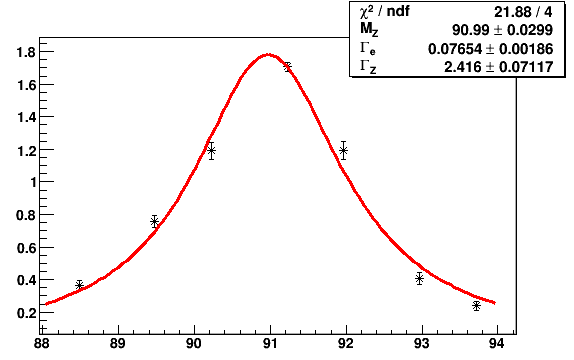
\includegraphics[width=0.49\textwidth]{../figures/elektronen.png}}
	\subfigure[Myonen]{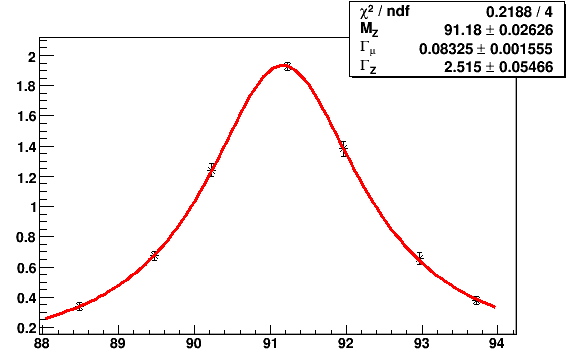
\includegraphics[width=0.49\textwidth]{../figures/myonen.png}}
	\subfigure[Tauonen]{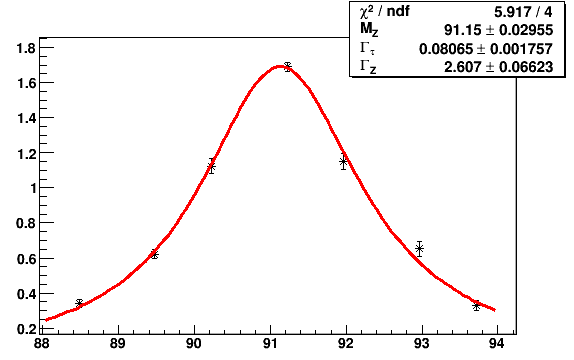
\includegraphics[width=0.49\textwidth]{../figures/tauonen.png}}
	\subfigure[Quarks]{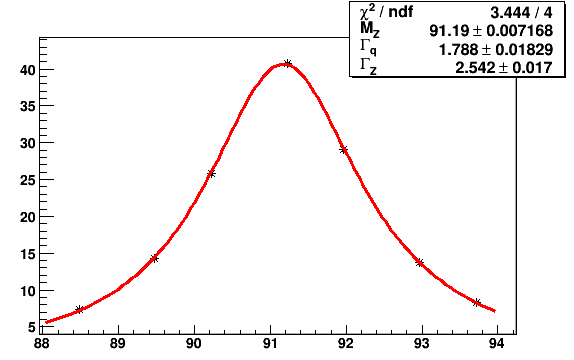
\includegraphics[width=0.49\textwidth]{../figures/quarks.png}}
	\subfigure[Leptonen]{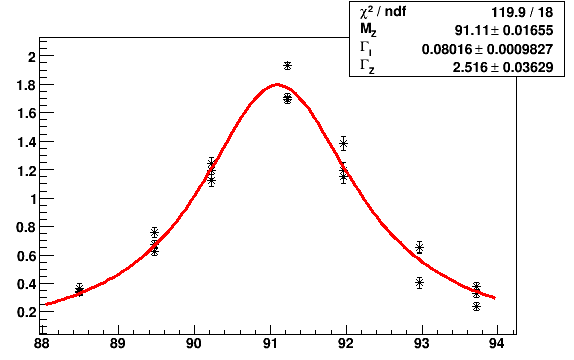
\includegraphics[width=0.49\textwidth]{../figures/leptonen.png}\label{fig:wirkungsquerschnitte:leptonen}}
	\subfigure[Leptonen (gewichtet)]{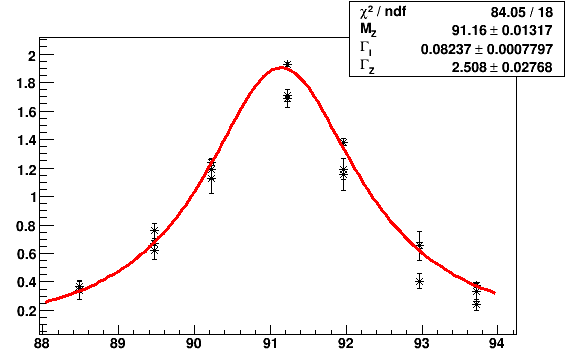
\includegraphics[width=0.49\textwidth]{../figures/leptonen_gewichtet.png}\label{fig:wirkungsquerschnitte:leptonengewichtet}}
	\caption[Wirkungsquerschnitte in Abhängigkeit der Schwerpunktsenergien]{Wirkungsquerschnitte in Abhängigkeit der Schwerpunktsenergien mit Fits zur Ermittelung der Z\textsuperscript0-Masse und der Partialbreiten.}
	\label{fig:wirkungsquerschnitte}
\end{figure}

Außerdem wurde unter der Annahme von Leptonenuniversalität (siehe Gleichung \ref{eq:leptonenuniversalitaet} in Abschnitt \ref{sec:partialbreiten}) in Abbildung \ref{fig:wirkungsquerschnitte:leptonen} die Partialbreite $\Gamma_{e/\mu/\tau}$ der Leptonen mit Hilfe der Daten aller leptonischen Zerfallskanäle bestimmt. Um die Qualität des Fits zu verbessern wurde eine Wichtung nach den $\frac{\chi^2}{\mathrm{ndf}}$-Werten der einzelnen Zerfallskanäle durchgeführt. Dies wurde solange wiederholt, bis der $\frac{\chi^2}{\mathrm{ndf}}$-Wert des gesamten Fits nicht mehr besser wurde. Das Ergebnis dieses gewichteten Fits ist in Abbildung \ref{fig:wirkungsquerschnitte:leptonengewichtet} dargestellt.

\subsubsection{Ergebnisse}

Als Ergebnis für die Gesamtzerfallsbreite $\Gamma_Z$ und die Masse $M_Z$ des $Z^0$-Bosons werden die Ergebnisse für den gewichteten Leptonenfit sowie für den Quarkfit gemittelt. Dabei erhalten wir folgende Ergebnisse:
\begin{alignat}{3}
	&M_Z^\text{Quarks}&&=&\,(91,190\pm0,007)\,\si{GeV}\text{,}\\
	&M_Z^\text{Leptonen}&&=&\,(91,160\pm0,013)\,\si{GeV}\text{,}\\
	&\Gamma_Z^\text{Quarks}&&=&(2542\pm17)\,\si{MeV}\text{,}\\
	&\Gamma_Z^\text{Leptonen}&&=&(2510\pm30)\,\si{MeV}\text{,}\\
	&M_Z&&=&\,(91,183\pm0,006)\,\si{GeV}\text{,}\\
	&\Gamma_Z&&=&(2534\pm15)\,\si{MeV}\text{.}
\end{alignat}

Für die leptonische Zerfallsbreite werden die Ergebnisse aus dem gewichteten leptonischen Fit verwendet. Für die leptonische und hadronische Zerfallsbreite ergeben sich folgende Ergebnisse:
\begin{alignat}{3}
	&\Gamma_{e/\mu/\tau}&&=&(82,4\pm0,8)\,\si{MeV}\text{,}\\
	&\Gamma_l&&=3\cdot\Gamma_{e/\mu/\tau}=\,\,&(247\pm2)\,\si{MeV}\text{,}\\
	&\Gamma_q&&=&(1788\pm18)\,\si{MeV}\text{.}
\end{alignat}

Für die Verzweigungsverhältnisse $\mathrm{BR}_f$ mit
\begin{align}
	\mathrm{BR}_f&=\frac{\Gamma_f}{\Gamma_Z}
\end{align}
erhalten wir folgende Ergebnisse:
\begin{alignat}{3}
	&\mathrm{BR}_l&&=&(9,7\pm1,0)\,\%\text{,}\\
	&\mathrm{BR}_\nu&&=&\,(19,7\pm0,9)\,\%\text{,}\\
	&\mathrm{BR}_q&&=&(70,6\pm0,8)\,\%\text{.}
\end{alignat}

\subsection{Bestimmung der Anzahl der Neutrinogenerationen}

Aus der Differenz zwischen der gesamten Zerfallsbreite $\Gamma_Z$ und der Summe der leptonischen und hadronischen Zerfallsbreiten $\Gamma_l+\Gamma_q$ lässt sich nun die unsichtbare Zerfallsbreite des Neutrino-Zerfallskanals bestimmen:
\begin{align}
	\Gamma_\nu&=\Gamma_Z-\left(\Gamma_l+\Gamma_q\right)=(500\pm20)\,\si{MeV}\text{.}
\end{align}

Aus Gleichung \ref{eq:neutrinos} in Abschnitt \ref{sec:partialbreiten} erhalten wir die Zerfallsbreite $\Gamma_{\nu_e/\nu_\mu/\nu_\tau}$ für eine einzelne Neutrinogeneration und berechnen damit aus der unsichtbaren Zerfallsbreite die Anzahl der Neutrinogenerationen:
\begin{align}
	N_\nu&=\frac{\Gamma_\nu}{\Gamma_{\nu_e/\nu_\mu/\nu_\tau}}=3,01\pm0,14\text{.}
\end{align}

\subsection{Bestimmung des Weinbergwinkels}

Zur Berechnung des Weinbergwinkels aus den gegebenen Daten des OPAL-Experiments verwenden wir die in Abschnitt \ref{sec:asymm} diskutierte Vorwärts-Rückwärts-Asymmetrie. Wir nutzen hierfür die Daten des myonischen Zerfallskanals. Zur Berechnung der Asymmetrie bestimmen wir aus den Messdaten die Summe aller Vorwärts-Ereignisse $\Sigma_\text{Vorwärts}=\cos\theta>0$ und die Summe aller Rückwärts-Ereignisse $\Sigma_\text{Rückwärts}=\cos\theta<0$ und berechnen die Asymmetrie folgendermaßen (vgl. Gleichung \ref{eq:asymm}):
\begin{align}
	A_\text{FB}&=\frac{\Sigma_\text{Vorwärts}-\Sigma_\text{Rückwärts}}{\Sigma_\text{Vorwärts}+\Sigma_\text{Rückwärts}}=0,077\pm0,018\text{.}
\end{align}

Daraus bestimmen wir mit Hilfe von Gleichung \ref{eq:weinberg} $\sin^2\theta_W$ folgendermaßen:
\begin{align}
	\sin^2\theta_W&=\frac14\left(1-\sqrt{\frac{A_{FB}}3}\right)=0,21\pm0,02\text{.}
\end{align}
Der Fehler berechnet sich hierbei mit Hilfe von Gauß'scher Fehlerfortpflanzung aus dem Poissonfehler auf die Ereignisanzahl.
	\newpage
	\section{Zusammenfassung und Diskussion}

Aus den experimentellen Daten des OPAL-Experiments haben wir die Wirkungsquerschnitte der verschiedenen Zerfallskanäle des Z\textsuperscript0-Bosons bei verschiedenen Schwerpunktsenergien bestimmt und daraus die partiellen und die gesamte Zerfallsbreite des Z\textsuperscript0-Bosons sowie seine Masse bestimmt. Dabei erhielten wir die in Tabelle \ref{tab:ergebnisse} beschriebenen und mit den in Abschnitt \ref{sec:partialbreiten} theoretisch berechneten Werten verglichenen Ergebnisse.\\

\begin{table}[bh]
	\centering
	\begin{tabular}{c|cc}
		&gemessener Wert&theoretischer Wert\\\hline
		$\Gamma_l\,/\,\si{MeV}$&$247\pm2$&$250,24\pm0,03$\\
		$\Gamma_q\,/\,\si{MeV}$&$1788\pm18$&$1674,59\pm0,19$\\
		$\Gamma_\nu\,/\,\si{MeV}$&$500\pm20$&$497,64\pm0,03$\\
		$\Gamma_Z\,/\,\si{MeV}$&$2534\pm15$&$2422,5\pm0,2$\\
		$M_Z\,/\,\si{GeV}$&$91,183\pm0,006$&$91,188\pm0,002$
	\end{tabular}
	\caption{Ergebnisse für Zerfallsbreiten und Z\textsuperscript0-Masse}
	\label{tab:ergebnisse}
\end{table}

Die Ergebnisse stimmen jeweils gut mit den theoretischen Werten überein, mit Ausnahme der hadronischen und der totalen Zerfallsbreite, welche höher als erwartet scheinen. Die Abweichung beträgt bei diesen beiden Werten ca. $5\,\sigma$. Möglicherweise ist diese Abweichung auf unsaubere Schnitte zurückzuführen. Außerdem waren die Schwerpunktsenergien des Detektors ohne Fehler angegeben. Wenn die Angaben der Energien nicht ganz den wahren Energien entsprechen, kann dies natürlich eine Verschiebung der Zerfallbreiten bewirken und führt zu einer zu geringen Fehlerabschätzung.\\

Außerdem wurden die Verzweigungsverhältnisse für geladene Leptonen, Hadronen und Neutrinos berechnet. Die Ergebnisse sind im Vergleich mit den in Abschnitt \ref{sec:partialbreiten} theoretisch berechneten Werten in Tabelle \ref{tab:branch} dargestellt.\\

\begin{table}[bh]
	\centering
	\begin{tabular}{c|cc}
		&gemessener Wert&theoretischer Wert\\\hline
		$\mathrm{BR}_l\,/\,\si{\%}$&$9,7\pm1,0$&$10,3298\pm0,0013$\\
		$\mathrm{BR}_q\,/\,\si{\%}$&$19,7\pm0,9$&$20,543\pm0,002$\\
		$\mathrm{BR}_\nu\,/\,\si{\%}$&$70,6\pm0,8$&$69,123\pm0,010$
	\end{tabular}
	\caption{Ergebnisse für Verzweigungsverhältnisse}
	\label{tab:branch}
\end{table}

Diese Werte stimmen innerhalb des Fehlers mit den theoretischen Verzweigungsverhältnissen überein.

Mit Hilfe der unsichtbaren Zerfallsbreite $\Gamma_\nu$ konnte die Anzahl der Neutrinogenerationen bestimmt werden (Literaturwert aus \cite{anleitungalt}):
\begin{alignat}{3}
	&N_\nu&&=&\,3,01\pm0,14\text{,}\\
	&N_\nu^\text{lit}&&=&3\text{.}
\end{alignat} 
Dies stimmt mit dem Literaturwert sehr gut überein.\\

Des Weiteren haben wir das Sinusquadrat des Weinbergwinkels $\sin^2\theta_W$ aus den Daten der Vorwärts-Rückwärts-Asymmetrie berechnet zu (Literaturwert aus \cite{nakamura}):
\begin{alignat}{4}
	&\sin^2\theta_W&&=&0,21\pm0,02\text{,}\\
	&\sin^2\theta_W^\text{lit}&&=&\,0,23116\pm0,00013\text{.}
\end{alignat}

Die Werte stimmen innerhalb von zwei Standardabweichungen überein, somit passt der gemessene Wert zur Theorie.

	\newpage
	\setcounter{section}{0}
	\renewcommand*{\thesection}{\Alph{section}}
	\section{Root-Skripte}
\label{sec:root}
\newpage
\section{R-Skripte}
\label{sec:r}
	\newpage
	\listoffigures
	\newpage
	\listoftables
	
	%Literatur----------------------------------------------------------------------------------------------------------
	
	%\cite{les}
	\newpage
	\printbibliography[heading=bibintoc]
	
%	\begin{thebibliography}{9}
%		
%		%\bibitem{staat}
%		%  Tobijas Kotyk,
%		%  \emph{Versuche zur Radioaktivität im Physikalischen Fortgeschrittenen Praktikum an der Albert-Ludwigs-Universität Freiburg},
%		%  Albert-Ludwigs-Universität, Freiburg,
%		%  2005
%		
%		
%		
%		%\bibitem{molmasse}
%		%  \emph{http://www.convertunits.com/molarmass/<ELEMENTNAME AUF ENGLISCH>}, Stand 28.09.2015
%		
%		
%		\bibitem{anleitung}
%		M. Köhli,
%		\emph{Versuchsanleitung Fortgeschrittenen Praktikum: SQUID},
%		Albert-Ludwigs-Universität Freiburg,
%		2011
%		
%		\bibitem{staat}
%		Volker Bange,
%		\emph{Einrichtung des Versuches "SQUID"},
%		Albert-Ludwigs-Universität Freiburg,
%		2000
%		
%		\bibitem{chemistry}
%		Bruce A. Averill, Patricia Eldredge,
%		\emph{General Chemistry: Principles, Patterns, and Applications},
%		Saylor Foundation,
%		2011
%		
%		\bibitem{SQUID}
%		Clarke, J.,
%		\emph{SQUIDS},
%		Spektrum der Wissenschaft , 10/1994,
%		Spektrum Akademischer Verlag
%	\end{thebibliography}
	
\end{document}